

\section{Related Work}
\label{sec:related_work}

\paragraph{Spatiotemporal Understanding in Vision Language Models}%
Vision Language Models (VLMs) have evolved rapidly by fully leveraging the significant achievements of Large Language Models (LLMs)~\cite{brown2020language, devlin2019bert, wei2021finetuned, bai2023qwen, touvron2023llama, radford2018improving} and large-scale visual instruction tuning datasets~\cite{liu2023visual, zhu2023minigpt, dai2023instructblip}. While VLMs~\cite{gong2023multimodal, liu2023visual, zhu2023minigpt, abouelenin2025phi4minitechnicalreportcompact, hurst2024gpt, li2024llava, team2024gemini, wang2024qwen2} exhibit transformative potential for applications such as embodied AI~\cite{suglia2024alanavlm, driess2023palm, kim2024openvla}, robotics~\cite{wang2024vlm, patel2025real}, and world modeling~\cite{liu2024world, zhang2024combo}, most existing methods remain constrained to static images, focusing narrowly on spatial understanding while overlooking the dynamic temporal dimension inherent in real-world interactions. To bridge this gap, emerging research~\cite{li2023videochat, zhang2023video, cheng2024videollama, maaz2023video, zhang2025videollama} has begun exploring video modality integration, aiming to equip VLMs with spatial-temporal awareness critical for tasks like video comprehension, where both contextual details and motion dynamics are essential. For example, VideoLLM-MoD~\cite{wu2024videollm} proposes to address the efficiency issue when processing long-term video by mixture-of-depths. ~\cite{yuan2024videorefer} introduces VideoRefer to enhance the finer-level (like object-level) spatial-temporal video understanding of VLMs. Grounded-VideoLLM~\cite{wang2024grounded} also targets for fine-grained video understanding through incorporating an additional temporal stream. In this work, we aim to rigorously evaluate the 4D spatial-temporal reasoning capabilities of state-of-the-art VLMs, probing how and to what extent these models internalize spatial intelligence and temporal dependencies.

\paragraph{VLM Benchmarks}% 
Following the development trends of VLMs, benchmarking VLMs shares the similar trajectory by first evaluating vision QA on static images~\cite{li2024seed, liu2024mmbench, he2024mmworld,yue2024mmmu}, to align with models’ early focus on 2D understanding. As VLMs evolved to tackle dynamic scenarios, benchmarks expanded to evaluate general-purpose video comprehension tasks that probe temporal coherence and event understanding~\cite{ning2023video, khattak2024good, li2024videoeval, fu2024video, li2024mvbench}. Notably, MMVU~\cite{zhao2025mmvu} further proposes a knowledge-intensive benchmark to assess the expert-level reasoning ability of current video-based large models. However, while these works assess perception and semantic understanding, they largely overlook the explicit evaluation of spatial-temporal awareness, a core capability for real-world applications requiring 4D (3D space + time) reasoning. Recent efforts like~\cite{yang2024thinking} pioneer benchmarks for 3D visual-spatial intelligence but restrict evaluation to static 3D scene, neglecting the interplay of object motion and temporal dynamics intrinsic to videos. In this work, we introduce \texttt{VLM4D}, the first benchmark designed to holistically evaluate the 4D intelligence in VLMs, unifying spatial understanding, temporal continuity, and motion reasoning. By curating tasks that demand precise analysis of dynamic interactions (e.g., direction prediction, perspective anticipation, and motion reasoning), \texttt{VLM4D} exposes critical gaps in current models' ability to internalize spatiotemporal relationships. Our work not only advances the granularity of VLM evaluation but also shares insights and potential solutions to improve the model performance.

\begin{figure*}[t]
    \centering
    % Replace 'example-image' with your image file name (e.g., 'myfigure.png')
    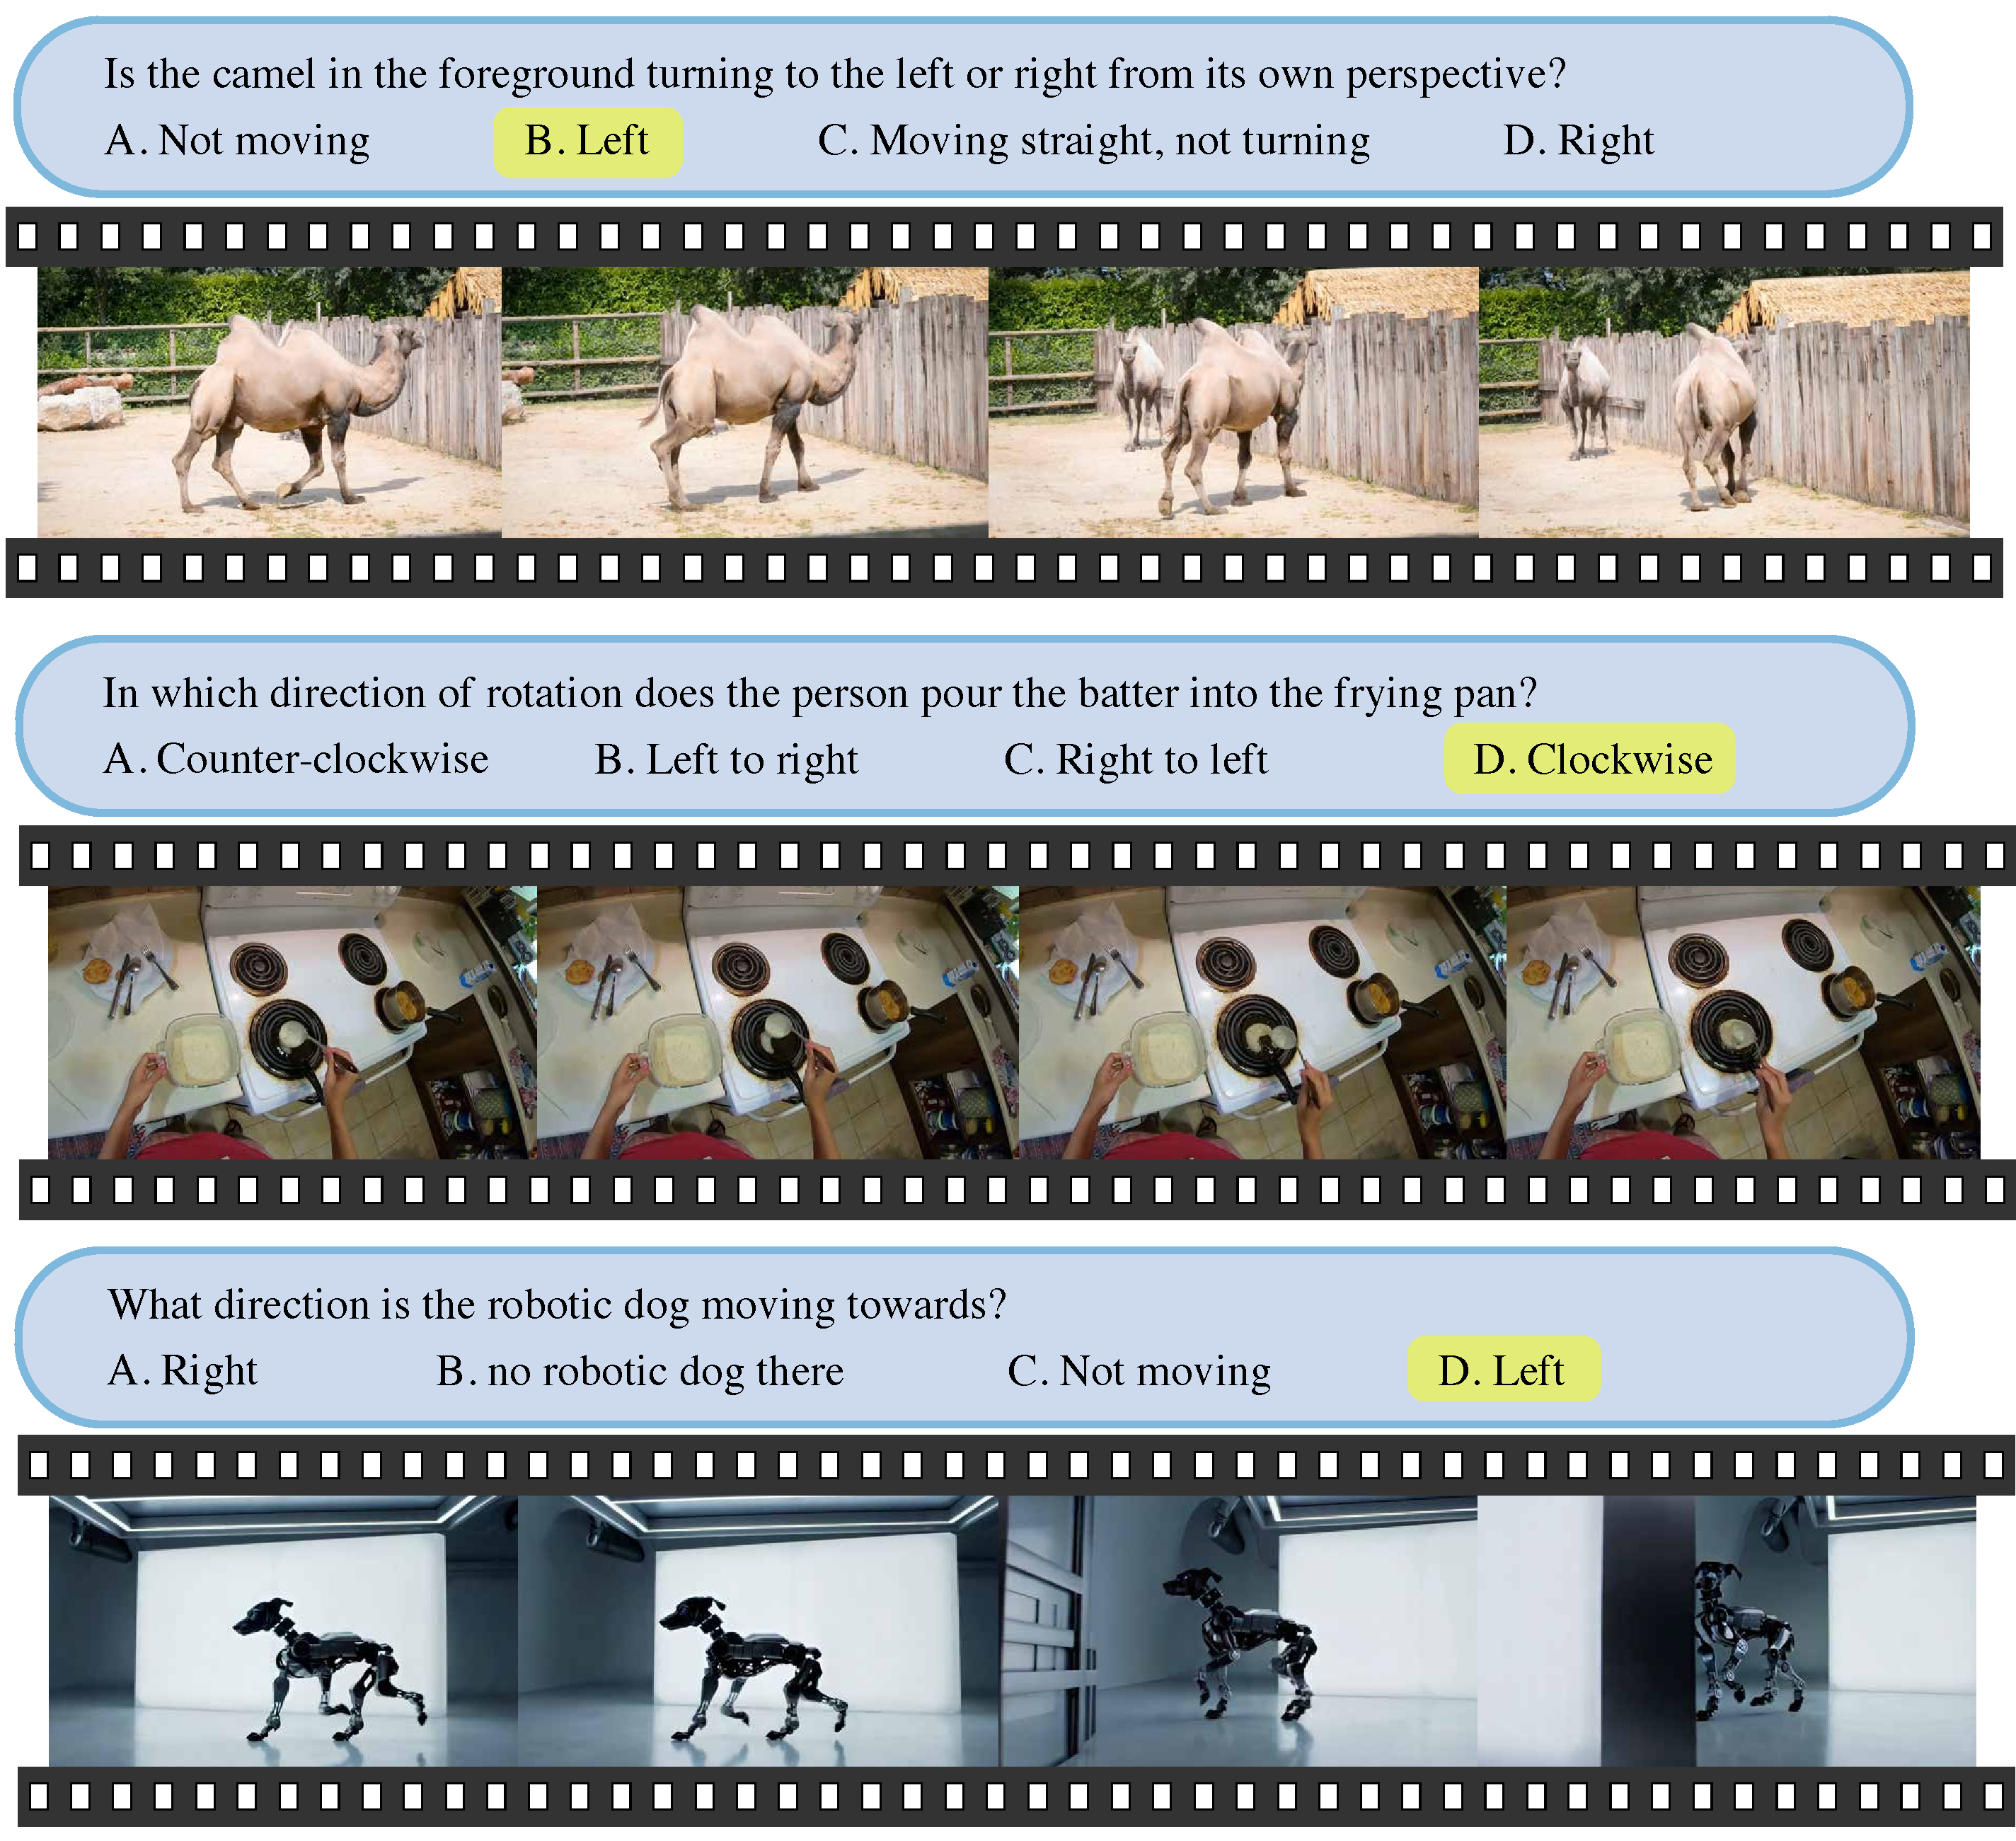
\includegraphics[width=0.8\textwidth]{figures/dataset_qualitative_v3.pdf}
    \caption{\textbf{Qualitative Examples of Dataset Annotations.} (Top) A third-person video with translational annotations (``camel turning left from its perspective"). (Middle) A first-person video with a rotational question (``clockwise rotation of ladle"). (Bottom) A synthetic scene with action recognition ``robotic dog moving right"). }
    \label{fig:qualitative_examples}
    \vspace{-0.5cm}
\end{figure*}